\subsection{Deep Dive: Mechanisms of Accelerated Transmission}
\label{sec:epidemic_deepdive}

The observation that structured networks yield higher and earlier peaks requires a rigorous analysis of the underlying network topology and initial conditions.
A primary driver for this acceleration is the degree-weighted initialization used for Model 1 and Model 2, where the first five infected individuals are selected with probabilities proportional to their degree \parencite{lloyd-smith2005superspreading}.
This setup reflects a realistic scenario where an outbreak is likely to be detected first among highly sociable "hubs" in the population.
As visualized in the left panels of Figure \ref{fig:network_metrics_baseline}, newly infected cases in Model 2 initially exhibit a significantly high mean degree, confirming that the pathogen rapidly exploits highly connected individuals during the early stages \parencite{salathe2010highresolution}.
Furthermore, human contact networks, particularly those in Model 2, are characterized by high degree assortativity, where individuals with many contacts tend to interact with other highly connected peers \parencite{newman2003mixing}.
In educational settings, school-aged children act as hubs that are densely connected within their own cohorts, facilitating an explosive, localized diffusion of the virus.
This localized intensity is quantitatively captured by the rapid spike in the proportion of infected contacts shown in the right panels of Figure \ref{fig:network_metrics_baseline} \parencite{salathe2010highresolution}.
While the Erd\H{o}s-R\'enyi model exhibits a smooth and gradual increase in local saturation, Model 1 and Model 2 show a much steeper rise \parencite{salathe2010highresolution}.
Because the pathogen is concentrated among hubs that are also connected to other hubs, the outbreak burns through these clusters rapidly, leading to the observed earlier peak and subsequent faster extinction of the overall epidemic \parencite{salathe2010highresolution}.

\begin{figure}[H]
    \centering
    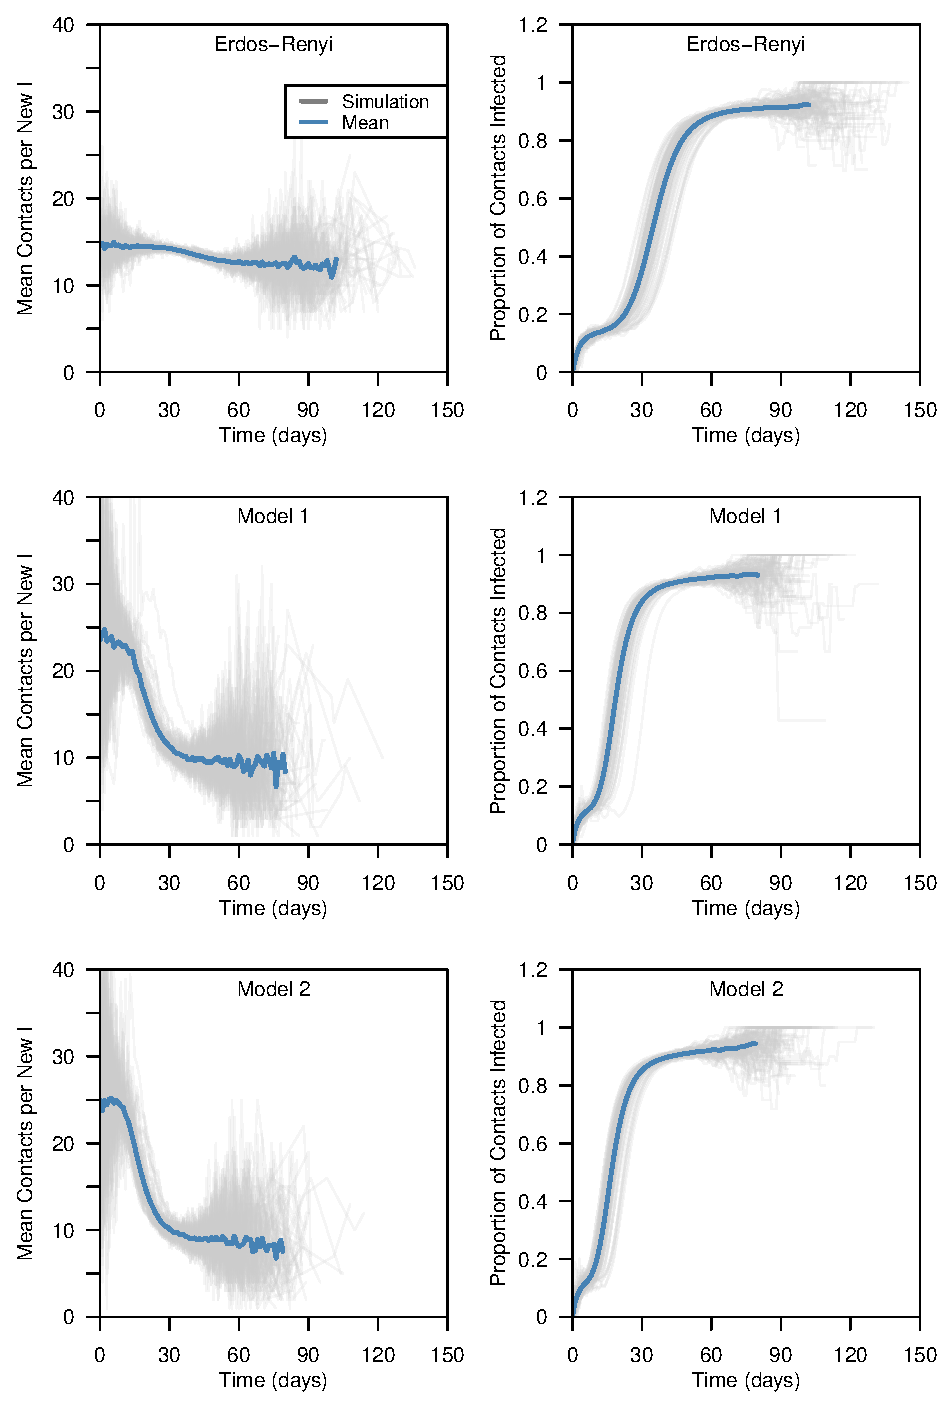
\includegraphics[width = 0.9\linewidth]{figures/04_EpidemicModel/network_metrics_baseline_3x2.pdf}
    \caption{Network metrics during the simulation. The earlier and higher peaks in structured models are explained by the early infection of hubs (left) and the resulting rapid local saturation within clustered cohorts (right).}
    \label{fig:network_metrics_baseline}
\end{figure}